% https://www.youtube.com/watch?v=ugpC98LcNqA
% https://www.youtube.com/watch?v=QrbhPcbZv0I

\section{Software architecture patterns}
Every non trivial software project should follow some architecture design.
But why? You want your project to be always maintainable and expandable as much easily as possible.
You want to modularize it, so that you can just take one part and exchange it without the need of rewriting the whole project.
And for this reason, there are architecture patterns.
I will describe three of them and explain my conclusion.

All of these three patterns have one thing in common.
They structure code into three main layers.
The names of those layers are present in these pattern's names.

\subsection{MVC}

\begin{figure}\centering
	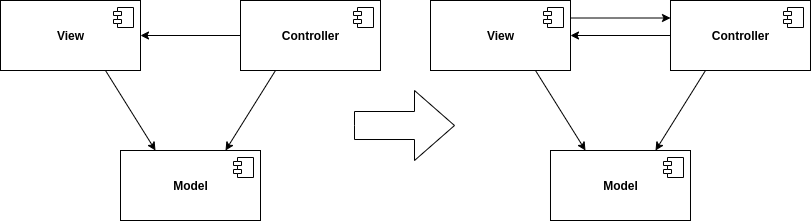
\includegraphics[width=1\textwidth]{pics/patterns/bc-mvc2.png}
	\caption[MVC]{Model View Controller}\label{fig:mvc}
\end{figure}

\textbf{Model View Controller}.
View is responsible for displaying data, controller is responsible for getting the user input and model for storing data.
The controller takes user input, it updates the model and then tells the view to update itself.

Now we know, that if we choose this, it will be implemented in android.
How does one do this? In the android world, the part of application responsible for displaying things is also responsible for dealing with user input.
So you tweak the pattern so the view gets the user input, it sends it to the controller, the controller updates the model, then tells the view to update itself, based on the data from model.

So both view and controller know the model, the view knows controller and controller knows view.
That's pretty bad, you don't want this.
That's high consistency and that is a thing you want to avoid, especially in the android world, where forgetting to remove a link can and will cause memory leaks.

And what if you want to somehow transform the data for presentation?
What part should do this presentation transformation, also known as UI logic?
You don't want to push this to the view, because you want the UI logic also to be easily testable and you want to separate it from the appearance of the view.
Controller can not posses it neither, because it doesn't supply any data to the view. So should you put it in the model? Absolutely not!
Why should a part of the application, responsible for data storing, know how to display stuff?

\subsection{MVP}

\begin{figure}\centering
	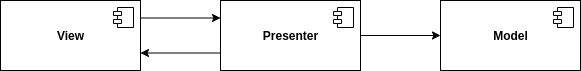
\includegraphics[width=0.7\textwidth]{pics/patterns/bc-mvp.png}
	\caption[MVP]{Model View Presenter}\label{fig:mvp}
\end{figure}

Imagine the MVC and the UI logic problem.
Now what if the view doesn't communicate with the model, but only with controller and the controller was also responsible for taking data from the model and supplying them to the view.
Then you would be able to put UI logic to this new controller. Now we will call it presenter, instead of new controller.
And that's what \textbf{Model View Presenter} is.

But that means the presenter still holds a link to the view. You still need to write some repetitive code because of this.
Second, why would the presenter should know, what parts of the view should be updated after the data changes?

\subsection{MVVM}

\begin{figure}\centering
	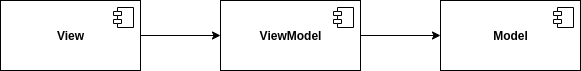
\includegraphics[width=0.7\textwidth]{pics/patterns/bc-mvvm.png}
	\caption[MVVM]{Model View ViewModel}\label{fig:mvvm}
\end{figure}

\textbf{Model View Viewmodel}.
We will borrow the MVP and tweak it a little. Currently the presenter knows the view and is executing it's methods when it needs to be updated.
Let's rename presenter to viewmodel. It no longer knows it's view.
Instead it provides some kind of stream and the view can observe the stream, so it can do whatever whenever it omits any data.

So the view knows the viewmodel, can call it's methods on user input and observe it's data streams.
The viewmodel knows model, observes it's data streams and omits them to the view.
The view knows the viewmodel, the viewmodel knows the model and the model don't know any of them.

\subsection{And the winner is ...}
Our choice is MVVM. Not only it looks like the tip of the evolution, but Google even made some libraries to support it.

\section{Main layers and libraries}
We will go over the three main layers of the MVVM, add a fourth at the end and describe some libraries that will be used inside of them.

\subsection{View}
As I said before, the view is the layer responsible for displaying data. It's what I call a screen in functional requirements.
The way it's implemented is through a combination of standard kotlin code and xml.
The xml is like a skeleton and kotlin is like life. In xml, you specify the look and in kotlin, you can specify what data it should display, how to update itself and what to do with user input.

For that, you have to somehow link or bind these two things (xml and kotlin) together.
We will be using a library called Data Binding. It's better than nothing and compared to other solutions, like kotlin's synthetics, Data Binding offers more features and I personally think it looks clearer.

\subsection{Viewmodel}
Google has made some architecture components and one of them is exactly for viewmodel.
It will be shame not to use it.

\subsection{Repository}
Repository will represent the model.
It's a place responsible for maintaining data.
Does the application need to download them, or load from cache?
Do you need to get anything out of the application or get anything in it?
You will ask the repository, also known as the one and the only source of truth.

\subsection{DAO and network IO}
This will be the fourth layer.
Every android app can run it's own LiteSQL database.
Data Access Objects will be used to access data in in this database.
There is a nice library for that called Room and we will be using it.
Network IO layer will be responsible for communication with server instance API.
We will be using Retrofit library for those API requests.
Repository will be using both of those in order to maintain and organise data.

\subsection{LiveData}
LiveData is a library.
It will be used in each layer.
Previously I talked about observing some kind of stream.
For this, you need some kind of observable variables and that's what LiveData is.
It enables you to set some action to happen when the data changes.
LiveData is now just some dumb stream, it only streams, when there is some observer living.
It may sound silly, but for example, you don't need to update certain screen, when that screen is not visible.

\section{Conclusion}

\begin{figure}\centering
	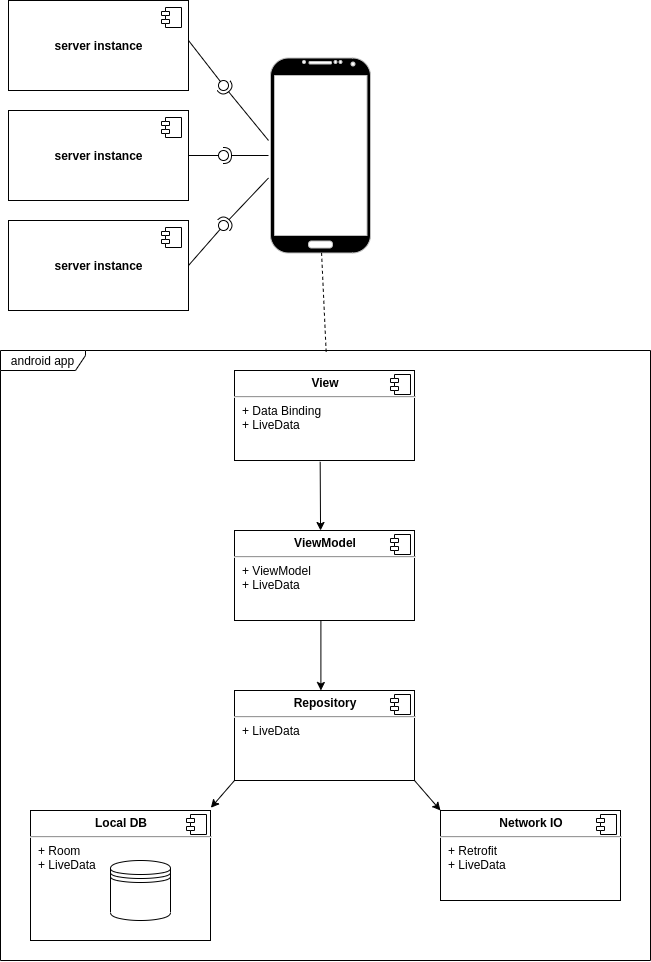
\includegraphics[width=1\textwidth]{pics/bc-architecture.png}
	\caption[Architecture]{Diagram consisting of MVVM and server instances}\label{fig:architecture}
\end{figure}

For better perspective, here is a summarizing diagram: \ref{fig:architecture}

The android device will communicate directly with multiple server instances. Network IO layer will be responsible for this communication. Repository will cache it using the Local DB layer and hand out data to the viewmodel. Viewmodel can do any UI logic that's needed and pass it to the view. All handing out or passing from any bottom layer to the one on top will be done through the observation of LiveData.